\section{Evaluation}

\subsection{Expressiveness}

In this section I want to answer part of my research question: \textit{"How can bug checkers be defined using finite automata with greater expressibility?"}. I show how monitor templates are more expressive compared to the the Computation Tree Logic (CTL) subset template formula found in EBA by providing examples of finite automata which cannot be expressed using the CTL template formula. It is worth noting that I am not comparing the entirety of CTL and monitor templates, but the subset of CTL used to define bug checkers found in EBA. 

In the implementation of the CTL template bug checker specifications by Abal et. al., the checkers implement four predicates, forming the CTL template formula of the shape $a\;\text{EU}\;(b\;\land\;EX\;(c\;\text{EU}\;d))$ \cite{Abal2017EffectiveBF}\cite{research-project}. This formula can also be written as $E\;a\;\text{U}\;(b\;\land\;EX\;(E\;c\;\text{U}\;d))$. This limits the expressiveness of checks which can be defined, given that the logic for detecting bugs must be implemented within these four functions $a$, $b$, $c$ and $d$. Specifying the checkers as monitor templates therefore allows for greater expressiveness in the checker definition. To illustrate this, Figure \ref{expressive-monitor} below shows a monitor template definition which cannot be defined in the existing CTL implementation of the EBA framework because there is no way to express the circular alternation.

\begin{figure}[H]
    \centering
    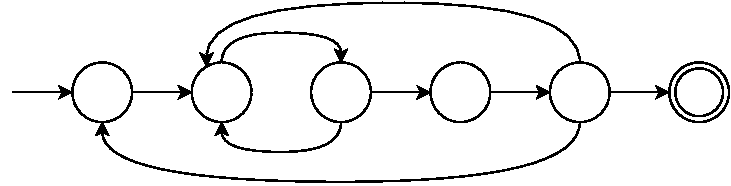
\includegraphics[width=0.5\textwidth]{evaluation/figures/monitor}
    \caption{An illustration of a monitor template which cannot be expressed by the CTL template formula $a\;\text{EU}\;(b\;\land\;EX\;(c\;\text{EU}\;d))$.}
    \label{expressive-monitor}
\end{figure}

\newpar Another example of a structure that the CTL template formulation cannot model is a very long sequence of given effects, e.g. an unlock and a lock repeatedly, followed by a final effect. This can be modelled using a monitor template defined as a loop between effects, going to the accepting state on the final effect. This is illustrated in Figure \ref{long-monitor}. 

\begin{figure}[H]
    \centering
    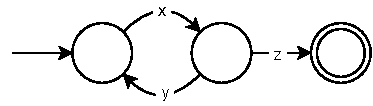
\includegraphics[width=0.35\textwidth]{evaluation/figures/long-monitor}
    \caption{An illustration of a monitor template which cannot be expressed by the CTL template formula $a\;\text{EU}\;(b\;\land\;EX\;(c\;\text{EU}\;d))$.}
    \label{long-monitor}
\end{figure}

\newpar I want to argue why this figure cannot be expressed in the CTL template. The CTL template has a shape with two EU operators, $a\;\text{EU}\;(...)$ and $c\;\text{EU}\;d$. Each of these operators enforce that the rightmost argument appears, but not necessarily the left, e.g. in $c\;\text{EU}\;d$ $d$ must appear while $c$ may or may not appear. Moreover, the left element can appear more than once. In the CTL template we only have two positions where we can enforce appearance and prevent repetition, on the righthand side of each $\text{EU}$. The monitor template in Figure \ref{long-monitor} requires strict alternation between any number of $x$ and $y$, so before any $y$ there is an $x$. Without a looping construct in the CTL template and only two positions where we force appearance and do not allow repetition, we can not express any alternations between repeating symbols of a length greater than two. 

\newpar On the other hand, the CTL template formula $a\;\text{EU}\;(b\;\land\;EX\;(c\;\text{EU}\;d))$ \textit{can} be expressed as a monitor template, as seen in Figure \ref{ctl-as-monitor}. 

\begin{figure}[H]
    \centering
    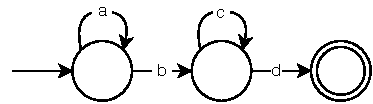
\includegraphics[width=0.35\textwidth]{evaluation/figures/ctl-as-monitor}
    \caption{An illustration of a monitor template equivalent to the CTL formula $a\;\text{EU}\;b\;\text{X}(c\;\text{EU}\;d)$.}
    \label{ctl-as-monitor}
\end{figure}

\newpar This expressiveness allows specifying the CTL template checkers defined in the work by Abal et. al and also possible future more granular checkers, in other words increasing the posibilities of extending the EBA framework. Certain bug types can show themselves in different code constructions, such as a double-unlock bug being defined as both an unlock happening before any locks happening and explicit double-unlocks. The expressiveness of monitor templates allows specifying multiple types of behaviour in the code under analysis for a single bug type as more complex transition function in order to increase the precision of checks.

\subsection{Accuracy}

In this section I want to answer the part of my research question: \textit{"How effective are such monitor template-based checker definitions?"}. I accomplish this by evaluating the implementation of a double-unlock bug checker using a monitor template on Linux kernel files known to contain double-unlock bugs. Effectiveness in this case means \textit{recall} since I am trying to detect actual positives in a set exclusively containing positives. Furthermore, the false positive rate is also a measure of effectiveness, since many false positives effectively reduce the overall quality of the output. Finding the precision of the double-unlock bug checker would require analysing all files in the Linux kernel and validating whether the reported positives are true or false positives by reading through and gaining an understanding for all files in the kernel --- a considerable undertaking consuming too much time.

Experimental static analysis has recently been added to the GCC compiler chain \cite{gcc10}, allowing developers to run check for double-free bugs in their code. David Malcolm --- the developer of the static analysis released in GCC 10 --- has described his challenges in reducing the amount of false positives during the development of the analysis \cite{gcc10-development}, showing that reducing these proves to be a difficult problem. Reducing false positives is important, since developers might avoid using a tool if they see false output too often. The developer of the popular \texttt{curl} command-line tool confirms this, noting that the addition of the analysis in GCC 10 is appreciated, but that it still produces too many false positives to be usable. \cite{curl-static-analysis}. Reducing the amount of false positives in the implementation of monitor templates has been difficult, since a tradeoff between the ability to detect more bugs and reducing the amount of false positives has to be made. In other words, increasing precision is hard. We see that the actual bugs are present, but false positives are also reported. 

\newpar The implementation has been evaluated by assembling a set of patched double-unlock bugs found in the Linux kernel source control, \textit{git}. Kernel developers submit patches as \textit{commits}, containing an message explaining what the patch addresses. These messages have been explored in search of the phrase \textit{"double unlock"}, resulting in 16 matching patches. These patches can be seen in Table \ref{evaluation-table}. These patches can be \textit{checked out} using git, in turn reverting the source code repository to the state where the patch was submitted. The source code repository can then be rolled back further to the commit just prior to the patch, in turn reverting the repository to a state where the bug is present. Once this has been done, the file under analysis can be compiled and analysed by the EBA framework with the implementation of the double-unlock checker. 

\newpar This process has been automated using the Docker tool in order to evaluate tests in a reproducable manner \cite{docker}. A base Linux Docker \textit{image} is used to provide the required Linux libraries for compilation and files are then compiled and extracted from this Docker image for analysis by EBA with and without the extensions described in this thesis. The results of analysis using the previous approach and my approach are then stored in text files for easy comparison for each file under analysis. 

\begin{table}[H]
    \centering
    \setlength{\tabcolsep}{5pt}
    \renewcommand{\arraystretch}{1.25}
    \scriptsize
    \begin{tabular}{llllllll}
    \textbf{Linux Kernel File}                    & \textbf{Lines} & \textbf{Patched in} & \textbf{Present in} & \textbf{Time} & \textbf{Mine} & \textbf{EBA} & \textbf{FP} \\
    \hline
    fs/ubifs/orphan.c                             & 1042           & \texttt{4dd75b33}   & \texttt{7542c6de}   & 1.03s         & +             & +            & 0           \\
    drivers/block/drbd/drbd\_main.c               & 3928           & \texttt{8e9c5230}   & \texttt{b0814361}   & 25.93s        & +             & -            & 6           \\
    drivers/gpu/drm/nouveau/nouveau\_svm.c        & 875            & \texttt{de4ee728}   & \texttt{5fbcf501}   & 0.97s         & -             & -            & 0           \\
    fs/btrfs/file.c                               & 3358           & \texttt{f49aa1de}   & \texttt{78e03651}   & 2.93s         & -             & -            & 0           \\
    drivers/staging/wilc1000/wilc\_wlan.c         & 1346           & \texttt{fea69916}   & \texttt{ca641bae}   & 1.26s         & +             & -            & 1           \\
    drivers/staging/kpc2000/kpc\_dma/fileops.c    & 420            & \texttt{c85aa326}   & \texttt{d4c596eb}   & 0.74s         & -             & -            & 0           \\
    fs/nfs/client.c                               & 1311           & \texttt{c260121a}   & \texttt{a46126cc}   & 1.79s         & -             & -            & 1           \\
    fs/btrfs/file.c                               & 3358           & \texttt{8fca9550}   & \texttt{2b90883c}   & 2.93s         & -             & -            & 0           \\
    drivers/media/dvb-core/dvbdev.c               & 1076           & \texttt{122d0e8d}   & \texttt{ded71626}   & 0.55s         & \%            & \%           & 0           \\
    mm/memory\_hotplug.c                          & 1867           & \texttt{e3df4c6e}   & \texttt{6376360e}   & 1.51s         & -             & -            & 0           \\
    sound/soc/codecs/pcm512x.c                    & 1721           & \texttt{28b698b7}   & \texttt{fd270fca}   & 1.06s         & -             & -            & 0           \\
    drivers/target/target\_core\_user.c           & 2735           & \texttt{f0e89aae}   & \texttt{807cf197}   & 0.82s         & \%            & \%           & 0           \\
    drivers/rpmsg/qcom\_smd.c                     & 1532           & \texttt{c3388a07}   & \texttt{fb416f69}   & 0.40s         & \%            & \%           & 0           \\
    drivers/scsi/aacraid/commsup.c                & 2615           & \texttt{d844752e}   & \texttt{09624645}   & 5.51s         & -             & -            & 2           \\
    drivers/staging/rtl8188eu/os\_dep/usb\_intf.c & 531            & \texttt{23bf4042}   & \texttt{612e1c94}   & -             & ?             & ?            & -           \\
    block/blk-cgroup.c                            & 1422           & \texttt{bbb427e3}   & \texttt{e0223003}   & -             & ?             & ?            & -           
    \end{tabular}
    \caption{The results of comparing the previous CTL-based approach to my monitor-template-based approach. The symbol \textbf{+} indicates that the bug was detected, \textbf{-} indicates that the bug was not detected, \textbf{\%} indicates an internal error in EBA and \textbf{?} indicates a compilation error. The column named FP indicates the number of false positives by the implementation using monitor templates reported in a file.}
    \label{evaluation-table}
\end{table}

\newpar The files \texttt{drbd\_main.c}, \texttt{orphan.c} and \texttt{wilc\_wlan.c} are successfully detected. Both of these files have a double-unlock in an if-statement which, when true, results in a double-unlock bug. In the case of the file \texttt{drbd\_main.c} by the use of mutexes, by a spin-unlock in the file \texttt{orphan.c}. 

\newpar The files \texttt{nouveau\_svm.c}, \texttt{fileops.c}, \texttt{file.c} and \texttt{memory\_hotplug.c} are not detected by either approach. These files exhibit a double-unlock bug when certain error codes are reported during execution, but unlocking happens by the use of an external function and is therefore not detected as an unlock by EBA.

\newpar The files \texttt{pcm512x.c} and \texttt{target\_core\_user.c} contain double mutex unlocks similar to \texttt{drbd\_main.c}, but these bugs are within static functions and are therefore ignored. The files \texttt{qcom\_smd.c} and \texttt{commsup.c} unlock using goto-statements, either resulting in EBA giving an internal error or not detecting the unlocks. 

\newpar EBA raises a stack overflow error on the file \texttt{dvbdev.c} and the remainder of the files \texttt{usb\_intf.c} and \texttt{blk-cgroup.c} fail to compile. A few reported positives in e.g. the file \texttt{commsup.c} seem like actual undiscovered double-unlock bugs, but given the complexity of the code under analysis I have been unable to verify whether these are in fact false positives or actual bugs. 

\newpar Remaining false positives are mainly reported in when an unlock is detected before the region the unlock happens on has been locked, as per the POSIX defintion of a double-unlock \cite{unlockPOSIX}. This is an unfortunate effect of the single-file analysis of EBA. Memory regions can have been unlocked elsewhere than the code under analysis if the file being analyses is part of a module consisting of several files. 

\newpar This evaluation has allowed me to answer part of my research question \textit{"How effective are such monitor template-based checker definitions?"}. The accuracy of the implementation of a double-unlock bug checker using monitor templates is higher than the previous approach. It is furthermore possible to express more complex bug checkers using monitor templates compared to the CTL template-based checker implementation, giving greater expressibility. In summary; though not all confirmed bugs are detected, a higher accuracy is observed when using monitor templates and monitor templates allow for greater expressibility when defining bug checkers. 